% =====================================================================
% Slide 11: Stage 5a -- composition NN surrogate
% =====================================================================
\begin{frame}{Stage 5a: Composition $\to (E, \nu)$ Neural Surrogate}
\begin{columns}[T]
\column{0.42\textwidth}
\textbf{Architecture.}
$12 \!\to\! 32 \!\to\! 20 \!\to\! 2$ fully-connected MLP\\
with ReLU activation; Huber loss on $\hat C_{11}, \hat C_{12}$;\\
deep ensemble of five seeds~\citep{lakshminarayanan2017}
for epistemic uncertainty.

\bigskip
\textbf{Held-out performance (30\,\% split):}
\begin{itemize}\small
  \item $R^{2}_{E} = 0.77$
  \item $R^{2}_{\nu} = 0.52$
\end{itemize}

\bigskip
\textbf{Validation on the Al\,7075 preset:}\\
$\hat E = 75.5$\,GPa,\ $\hat \nu = 0.334$\\
\scriptsize (published reference: $71{-}72$\,GPa,\ $\nu \approx 0.33$).

\bigskip
\scriptsize\textit{Distributed as a portable application image.}

\column{0.56\textwidth}
\centering
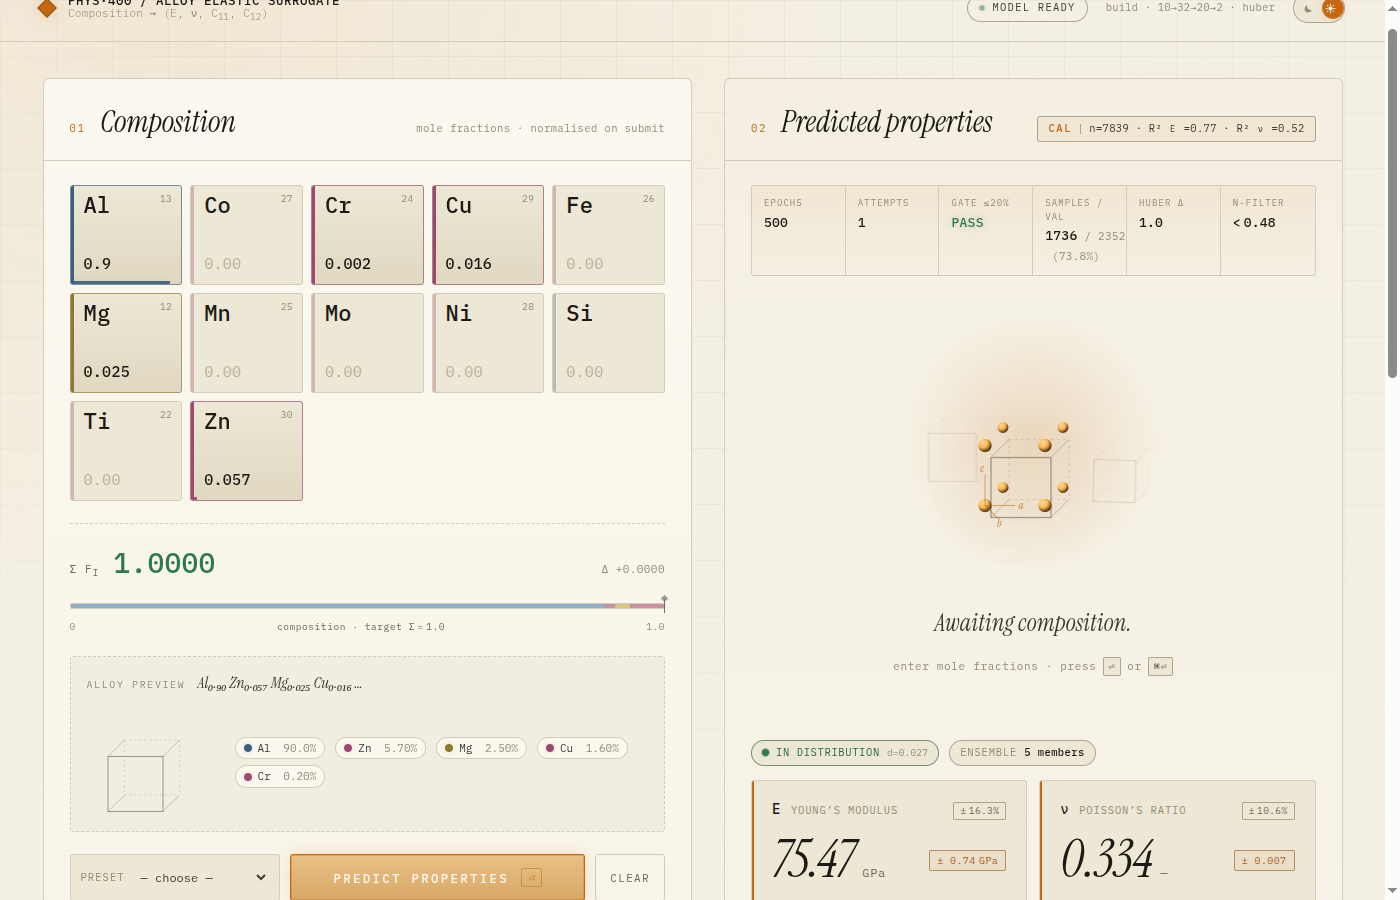
\includegraphics[width=0.99\linewidth]{figures/ml_app.png}\\[-0.2em]
\scriptsize Interactive composition predictor with $k$-nearest-neighbour
distance-based out-of-distribution flagging.
\end{columns}
\end{frame}
